\documentclass[12pt,a4paper,notitlepage]{article}
% \documentclass[conf]{new-aiaa}
\usepackage[framed,numbered,autolinebreaks]{mcode}
\usepackage[margin=1in]{geometry}
\usepackage{amsmath}
\usepackage{amsfonts}
\usepackage{amssymb}
\usepackage{graphicx}
\usepackage{color}
\usepackage{float}
\usepackage[toc,page]{appendix}
\usepackage{parskip}
\usepackage{sectsty}
\usepackage{gensymb}
\usepackage{titlesec}
\usepackage{listings}
\usepackage{titling}
\setlength{\droptitle}{-1cm}
\usepackage{enumitem}
\usepackage{multirow}
\usepackage{longtable}

\usepackage[
backend=biber,
style=numeric,
sorting=none
]{biblatex}
 
\addbibresource{draft.bib}


\setlist[enumerate]{topsep=0pt,itemsep=-3.5ex,partopsep=1ex,parsep=1ex}
\renewcommand{\rmdefault}{ptm}
\sectionfont{\fontsize{12}{0}\selectfont}
\subsectionfont{\fontsize{12}{0}\selectfont}
\usepackage[font={normal,bf}]{caption}

% Header and Footer
\setlength{\headheight}{15pt} 
\usepackage{fancyhdr}
\fancypagestyle{plain}{
 \fancyhf{}
 \fancyhead[L]{AA 290: AA 279D Project}
 \fancyhead[R]{Stanford University}
 \fancyfoot[C]{\thepage}
}

% Table of contents
\setcounter{tocdepth}{5}

\begin{document}
\title{\Huge \textbf{Project Title}}
\author{\Large Ethan LeBoeuf}
\date{\Large 23 September 2019}

\begin{minipage}[h]{\textwidth}
	\vspace{4 cm}
	\advance\leftskip-1in
    \maketitle
\end{minipage}

\begin{figure}[H]
\centering
\includegraphics[scale=0.28]{Images/SOHO.jpg}
\end{figure}

\pagebreak

\section*{\Large REVISION HISTORY}

\begin{table}[h!]
\begin{center}
\begin{tabular} [0.9 \textwidth]{cl}
\hline \hline
\multicolumn{1}{c}{VERSION} & \multicolumn{1}{l}{REVISION NOTES} \\
\hline
PS1 & - Created document \\
    & - Added PS1 material \\
%  \hline
%  PS2 & - Added PS2 material \\
%  & - Updated title page \\
%  & - Added table of contents \\
%  & - Updated orbit around L2 point \\
%  & - Discretized cylindrical parts of geometry \\
\hline \hline
\end{tabular}
	\caption{Summary of project revisions.}
\end{center}
\end{table}
 
\newpage
\section*{\Large TABLE OF CONTENTS}
\makeatletter
\@starttoc{toc}
\makeatother
\newpage
%%%%%%%%%%%%%%%%%%%%%%%%%%%%%%%%%%%%%%%%%%%%%%%%%%%%%%%%%%%%%%%%%%%%%%%%%%%%%%%%%%%%%%%%%%%%%%%%%%%%%%%%%%%%%%%%%%%%%%%%%%%%%%%%%%%%%%%%%%%%%%%%%%%%%%%%%%%%%%%%%%%%%%%%%%%%%%%%%%%%%%%%%%%%%%%%%%%%%%%%%%%%%%%%%%%%%%%%%%%

% \section{\Large INTRODUCTION}

\section{\Large PROBLEM SET 1}
\subsection{PROBLEM 1}
\textit{Select the characteristics of your mission}

For our project, we have decided to pursue an interplanetary, and sun pointing target attitude satellite mission. The attitude will be parameterized using quaternions, as they are widely used for attitude dynamics of spacecraft. Quaternions provide a few distinct advantages such as, no singularity and a lower computational expense as compared to other parameterization methods (i.e. Euler angles and direction cosines). The primary sensor type used to determine the orientation will be gyroscopes. Attitude actuation will be controlled by spinning up or braking down three reaction wheels.

\subsection{PROBLEM 2}
\textit{Conduct survey of satellites which have characteristics similar to selected project. Use internet,
publications, and books as resources.}

In order to select a mission that met our desired characteristics, various solar-focused satellite missions were surveyed. A majority of the solar-based missions researched featured an orbit around one of the Sun-Earth Lagrange points (location where an object is suspended between the Sun and Earth gravitational fields), a heliocentric orbit, or a high altitude Earth orbit.

The first mission to utilize an L1 Lagrange point orbit was the International Cometary Explorer (ISEE-3), launched on August 12, 1978. This mission verified the usage of Lagrange points for trajectory planning. It was also the first usage of a halo orbit, a periodic, three dimensional orbit near L1, L2, and L3 orbits.

Another solar observation mission that featured a halo orbit around the L1 Lagrange point, was the Solar and Heliospheric Observatory (SOHO) mission. This mission was launched on December 2, 1995 as a joint project between NASA and the ESA, and primary focus was to observe the outer layer and interior structure of the Sun. The SOHO mission is distinct, as it has led to the inadvertent discovery of over 2000 comets. It was also the first three-axis-stabilized spacecraft to operate without a gyroscope, after an on-board failure of gyroscope led to the use of the reaction wheels as a virtual gyroscope.

The Deep Space Climate Observatory (DSCOVR) mission, launched on February 11, 2015, is a spacecraft that observes both the Sun and the Earth, for solar mind monitoring and Earth climate phenomena respectively. DSCOVR also orbits the L1 Lagrange point similar to SOHO, although in a Lissajous orbit, which is similar to halo orbits, but is quasi-periodic.

The Solar Dynamics Observatory (SDO), which launched on February 11, 2010, is another solar monitoring spacecraft primarily concerned with the effect of dynamic solar activity on Earth. Instead of orbiting a Sun-Earth Lagrange point, SDO was placed in a a geosynchronous, circular orbit around Earth. This greatly reduces the complexity of the attitude maneuvers of the mission, as the pointing of the spacecraft's antenna towards Earth for communications is constant for a geosynchronous orbit.

Another solar pointing spacecraft is the Solar Terrestrial Relations Observatory (STEREO). However, the STEREO mission is distinct from SOHO in that it features two identical spacecraft, which were placed in heliocentric orbits with different orbital periods. The dual spacecraft gradually pull farther ahead of and fall behind of the Earth respectively, have passed through the L4 and L5 Lagrange points, and have no defined final positions.

\subsection{PROBLEM 3}
\textit{Select preferred existing satellite and payload for project. Similarity is helpful, but not strictly required.}

We chose to model our mission after the Solar and Heliospheric Observatory (SOHO) mission. The SOHO Payload Module features twelve instruments used for both independent and synchronized observation of the sun, in addition to other critical spacecraft components. The instruments are listed below:
\begin{enumerate}
    \item Coronal Diagnostic Spectrometer (CDS)
    \newline
    \item Charge Element and Isotope Analysis System (CELIAS)
    \newline
    \item Comprehensive Suprathermal and Energetic Particle Analyser Collaboration (COSTEP)
    \newline
    \item Extreme Ultraviolet Imaging Telescope (EIT)
    \newline
    \item Energetic and Relativistic Nuclei and Electron Experiment (ERNE)
    \newline
    \item Global Oscillations at Low Frequencies (GOLF)
    \newline
    \item Large Angle and Spectrometric Coronagraph (LASCO)
    \newline
    \item Michelson Doppler Imager (MDI)
    \newline
    \item Solar Ultraviolet Measurement of Emitted Radiation (SUMER)
    \newline
    \item Solar Wind Anisotropies (SWAN)
    \newline
    \item Ultraviolet Coronagraph Spectrometer (UVCS)
    \newline
    \item Variability of Solar Irradiance and Gravity
    Oscillations (VIRGO)
    \newline
\end{enumerate}

\subsection{PROBLEM 4}
\textit{Collect basic information on mission, requirements, ADCS sensors and actuators, mechanical layout, mass,
mass distribution, and inertia properties.}

The initial, primary scientific objectives of the SOHO mission were to observe the solar corona (the outer layer), investigate solar wind production, and examine the structure and dynamics of the Sun's interior. After the mission's inception, SOHO has also been used for comet discovery by blocking out the Sun's glare. SOHO maintains a trajectory around the Sun, in step with the Earth, by orbiting the First Lagrange Point (L1). SOHO is a three-axis stabilized spacecraft that is constantly facing the Sun.

For the mission, the ADCS featured gyroscopes for sensing and three reaction wheels in addition to a thruster for actuation. During the mission there was a failure of the gyroscopes which we hope to try and consider for this project as well. 

The base of the spacecraft, also known as the service module, houses vital spacecraft components such as, thrusters, power, and communications. The payload module is attached to service module, and contains the aforementioned twelve instrument packages for solar observation. The solar panels are deployed at the base of the spacecraft, extending its total width to 9.5 m. 

The outer dimensions of the spacecraft are 4.3 m (height) x 2.7 m (breadth) x 9.5 m (width). At launch, the mass of the spacecraft was 1,850 kg, and the payload mass is 610 kg.

\subsection{PROBLEM 5} \label{geometry}
\textit{Simplify spacecraft geometry, make assumptions on mass distribution, e.g. splitting it in its core parts,
define body axes (typically related to geometry and payload), compute moments of inertia and full inertia
matrix w.r.t. body axes.}

In order to simplify the geometry, SOHO was broken down into three main components; the base, the solar panels, and the scientific payload section. The solar panels are affixed to the sides of the base section, and the scientific payload section is affixed on top of the base. A model of this simplified geometry is shown in Figure \ref{fig:SOHO_simple}.

\begin{figure}[H]
  \centering
    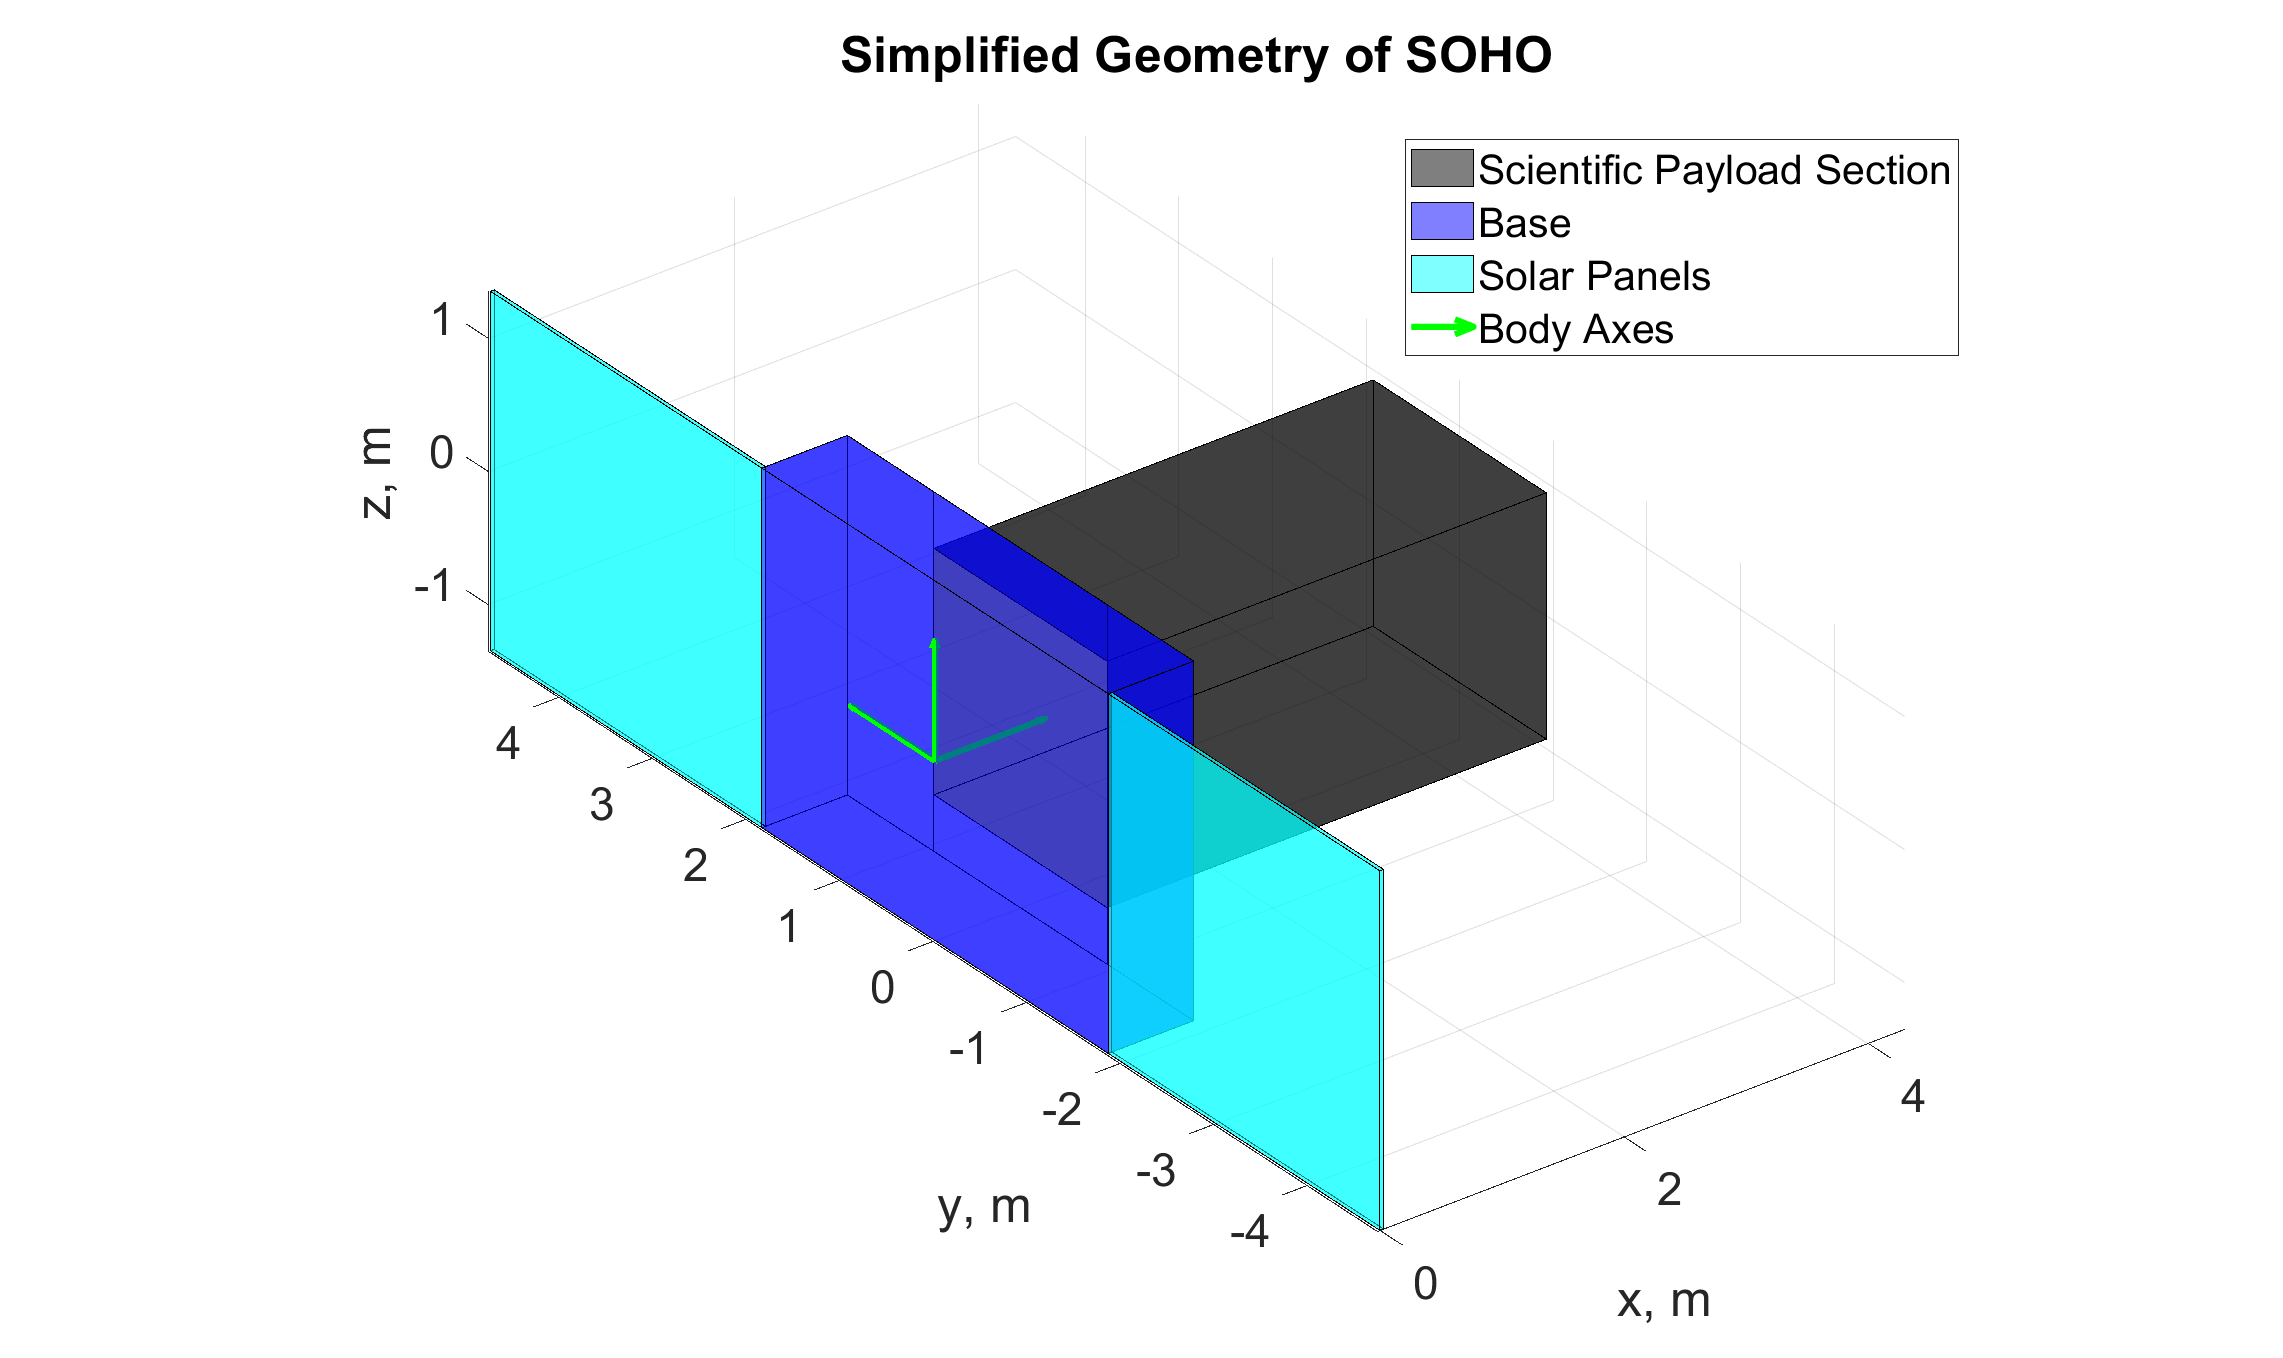
\includegraphics[width=\textwidth]{Images/SOHO_plain.eps}
  \caption{The simplified geometry for SOHO.}
  \label{fig:SOHO_simple}
\end{figure}

The body axes were selected based on the NASA's conventions for the axes of rotation, as found on the official SOHO mission website \cite{website:soho_nasa}, which can be seen Figure \ref{fig:SOHO_conv}.

\begin{figure}[H]
  \centering
    \includegraphics[width=.5\textwidth]{Images/SOHOconv.jpg}
  \caption{NASA axes of rotation for SOHO \cite{website:soho_nasa}.}
  \label{fig:SOHO_conv}
\end{figure}

In order to calculate the moments of inertia, it was assumed that each section in our simplified geometry had a uniform density. The respective masses and dimensions of each section can be found in Table \ref{table:dimensions}

\begin{table}[h!]
\begin{center}
\begin{tabular}{ |c||c|c|c|c|}
 \hline
 \multicolumn{5}{||c||}{\textbf{Simplified Geometry Section Masses and Dimensions}} \\
 \hline
 \textit{Sub-System}& \textit{Mass} ($kg$) &\textit{Width} ($m$)&\textit{Breadth} ($m$) &\textit{Height} ($m$)\\
\hline
Base Section& 1144.107 & 3.7 & 2.7 & 0.7 \\ 
\hline
Solar Panel (2)& 47.947 & 2.9 & 2.7 & 0.03 \\ 
\hline
Payload Section& 610 & 3.7 & 2.7 & 0.7 \\ 
\hline
\end{tabular}
\caption{Mass and geometric dimensions of each SOHO subsection.}
\label{table:dimensions}
\end{center}
\end{table}

Using these properties, inertia tensor, shown below, was calculated in Matlab. The code for this calculation can be found in \ref{A:P1p5}.

\begin{equation}
I_{B} =
\begin{bmatrix} 
I_{xx} & -I_{xy} & -I_{xz} \\
-I_{yx} & I_{yy} & -I_{yz} \\ 
-I_{zx} & -I_{zy} & I_{zz} \\
\end{bmatrix}
 =
\begin{bmatrix}
3517.982 & 0 & 0 \\
0 & 5585.477 & 0 \\ 
0 & 0 & 7248.903 \\
\end{bmatrix}
[kg/m^2].
\end{equation}

Based on the geometry simplification and the location of the body axes, the x-z and x-y planes are symmetric, which make all the product of inertia terms equal to zero.

\subsection{PROBLEM 6} \label{principal_axes}
\textit{In general the body axes are not the principal axes. Identify principal axes through the
eigenvector/eigenvalue problem discussed in class and compute the rotation matrix from body to principal
axes.}

The body axes and principal axes are co-located, as shown by the inertia tensor w.r.t the principal axes below, which is identical to the inertia tensor w.r.t. the body axes.
\begin{equation}
I_{P} =
\begin{bmatrix} 
I_{x'} & 0 & 0 \\
0 & I_{y'} & 0 \\ 
0 & 0 & I_{z'} \\
\end{bmatrix}
 =
\begin{bmatrix}
3517.982 & 0 & 0 \\
0 & 5585.477 & 0 \\ 
0 & 0 & 7248.903 \\
\end{bmatrix}
[kg/m^2].
\end{equation}

This was confirmed using Matlab's eigenvalue/eigenvector function; this calculation can be found in \ref{A:P1p5}. Since the principal axes are identical to the body axes, no rotation matrix is needed. Typically, principal axes are aligned at the spacecraft center of mass, so this change will potentially occur in the future by translating both the body axes and principal axes to the COM. Since the x-z and x-y planes are symmetric, the principal axes will only need to be translated along the x-axis.


% \begin{figure}[H]
% \centering
% \includegraphics[scale=0.7]{./WMAP_CAD4.PNG}
% \caption{A 3D model of the simplified satellite geometry. The body and principal axes are labeled and located at the spacecraft center of mass.}
% \label{CAD model with frames}
% \end{figure}


% \begin{equation}
% \vec{M} = \vec{I} \cdot \vec{\dot{\omega}}\ + \vec{\omega} \times \vec{I} \cdot \vec{\omega} \\ 
% \end{equation}   



% \begin{eqnarray}
% M_x = I_{xx} \dot{\omega_x} + (I_{zz} - I_{yy})\omega_y \omega_z \nonumber \\
% M_y = I_{yy} \dot{\omega_y} + (I_{xx} - I_{zz})\omega_z \omega_x \\
% M_z = I_{zz} \dot{\omega_z} + (I_{yy} - I_{xx})\omega_x \omega_y \nonumber
% \end{eqnarray}


\subsection{PROBLEM 7}
\textit{Discretize your spacecraft through its outer surfaces (geometry). Develop a Matlab/Simulink function to handle barycenter (geometry, no mass distribution) coordinates, size, and unit vectors normal to each outer surface of the spacecraft in body frame.}

To complete this problem, the simplified geometric features were represented in Matlab using nested structures. The overall structure contained the structures of each main section of the spacecraft. Each of these subsections structures contained structures for the outward faces. The face structure captured the coordinates, barycenter, area, and normal vector for each face on the simplified spacecraft. This information can be seen in Table \ref{table:discrete}. A visual representation of the discretized spacecraft can be seen in Figure \ref{fig:SOHO_disc}. The code used to generate these values and the figure can be found in \ref{A:P1p7}.

\begin{table}[H]
\begin{center}
\begin{tabular}{ |p{1.5cm}||p{1.5cm}|p{2cm}|p{4cm}|p{3cm}|}
 \hline
 \multicolumn{5}{|c|}{\textbf{Spacecraft Discretization}} \\
 \hline
 Sub-System& Face \#&Area ($m^2$)&Barycenter Coordinates&Unit Normal\\
\hline
\multirow{5}{2em}{Payload Section} & 1 & 3.4225 & [4.3, 0, 0]&[1, 0, 0]\\ 
& 2 & 6.6600 & [2.5, 0.925, 0]&[0, 1, 0] \\ 
& 3 & 6.6600 & [2.5, 0, 0.925] &[0, 0, 1]\\ 
& 4 & 6.6600 & [2.5, -0.925, 0] &[0, -1, 0]\\
& 5 & 6.6600 & [2.5, 0, -0.925] &[0, 0, -1]\\
\hline
\multirow{9}{2em}{Base} & 1 & 9.9900 & [0, 0, 0]&[-1, 0, 0]\\ 
& 2 & 1.8090 & [0.365, 1.85, 0] &[0, 1, 0]\\ 
& 3 & 1.8090 & [0.365, -1.85, 0] &[0, -1, 0]\\ 
& 4 & 2.5900 & [0.35, 0, 1.35] &[0, 0, 1]\\
& 5 & 2.5900 & [0.35, 0, -1.35] &[0, 0, -1]\\
& 6 & 2.4975 & [0.7, -1.3875, 0]&[1, 0, 0] \\
& 7 & 2.4975 & [0.7, 1.3875, 0] &[1, 0, 0]\\
& 8 & 0.7863 & [0.7, 0, 1.1375] &[1, 0, 0]\\
& 9 & 0.7863 & [0.7, 0, -1.1375] &[1, 0, 0]\\
\hline
\multirow{5}{2em}{Solar Panel 1} & 1 & 7.8300 & [0, 3.3, 0]&[-1, 0, 0]\\ 
& 2 & 7.8300 & [0.03, 3.3, 0] &[1, 0, 0]\\ 
& 3 & 0.0810 & [0.015, 4.75, 0]&[0, 1, 0] \\ 
& 4 & 0.0870 & [0.015, 3.3, 1.35]&[0, 0, 1] \\
& 5 & 0.0870 & [0.015, 3.3, -1.35]&[0, 0, -1] \\
\hline
\multirow{5}{2em}{Solar Panel 2} & 1 & 7.8300 & [0, -3.3, 0]&[-1, 0, 0]\\ 
& 2 & 7.8300 & [0.03, -3.3, 0]&[1, 0, 0] \\ 
& 3 & 0.0810 & [0.015, -4.75, 0] &[0, -1, 0]\\ 
& 4 & 0.0870 & [0.015, -3.3, 1.35] &[0, 0, 1]\\
& 5 & 0.0870 & [0.015, -3.3, -1.35] &[0, 0, -1]\\
\hline
\end{tabular}
\caption{Area and barycenter coordinates for each face on the discretized spacecraft.}
\label{table:discrete}
\end{center}
\end{table}

\begin{figure}[H]
  \centering
    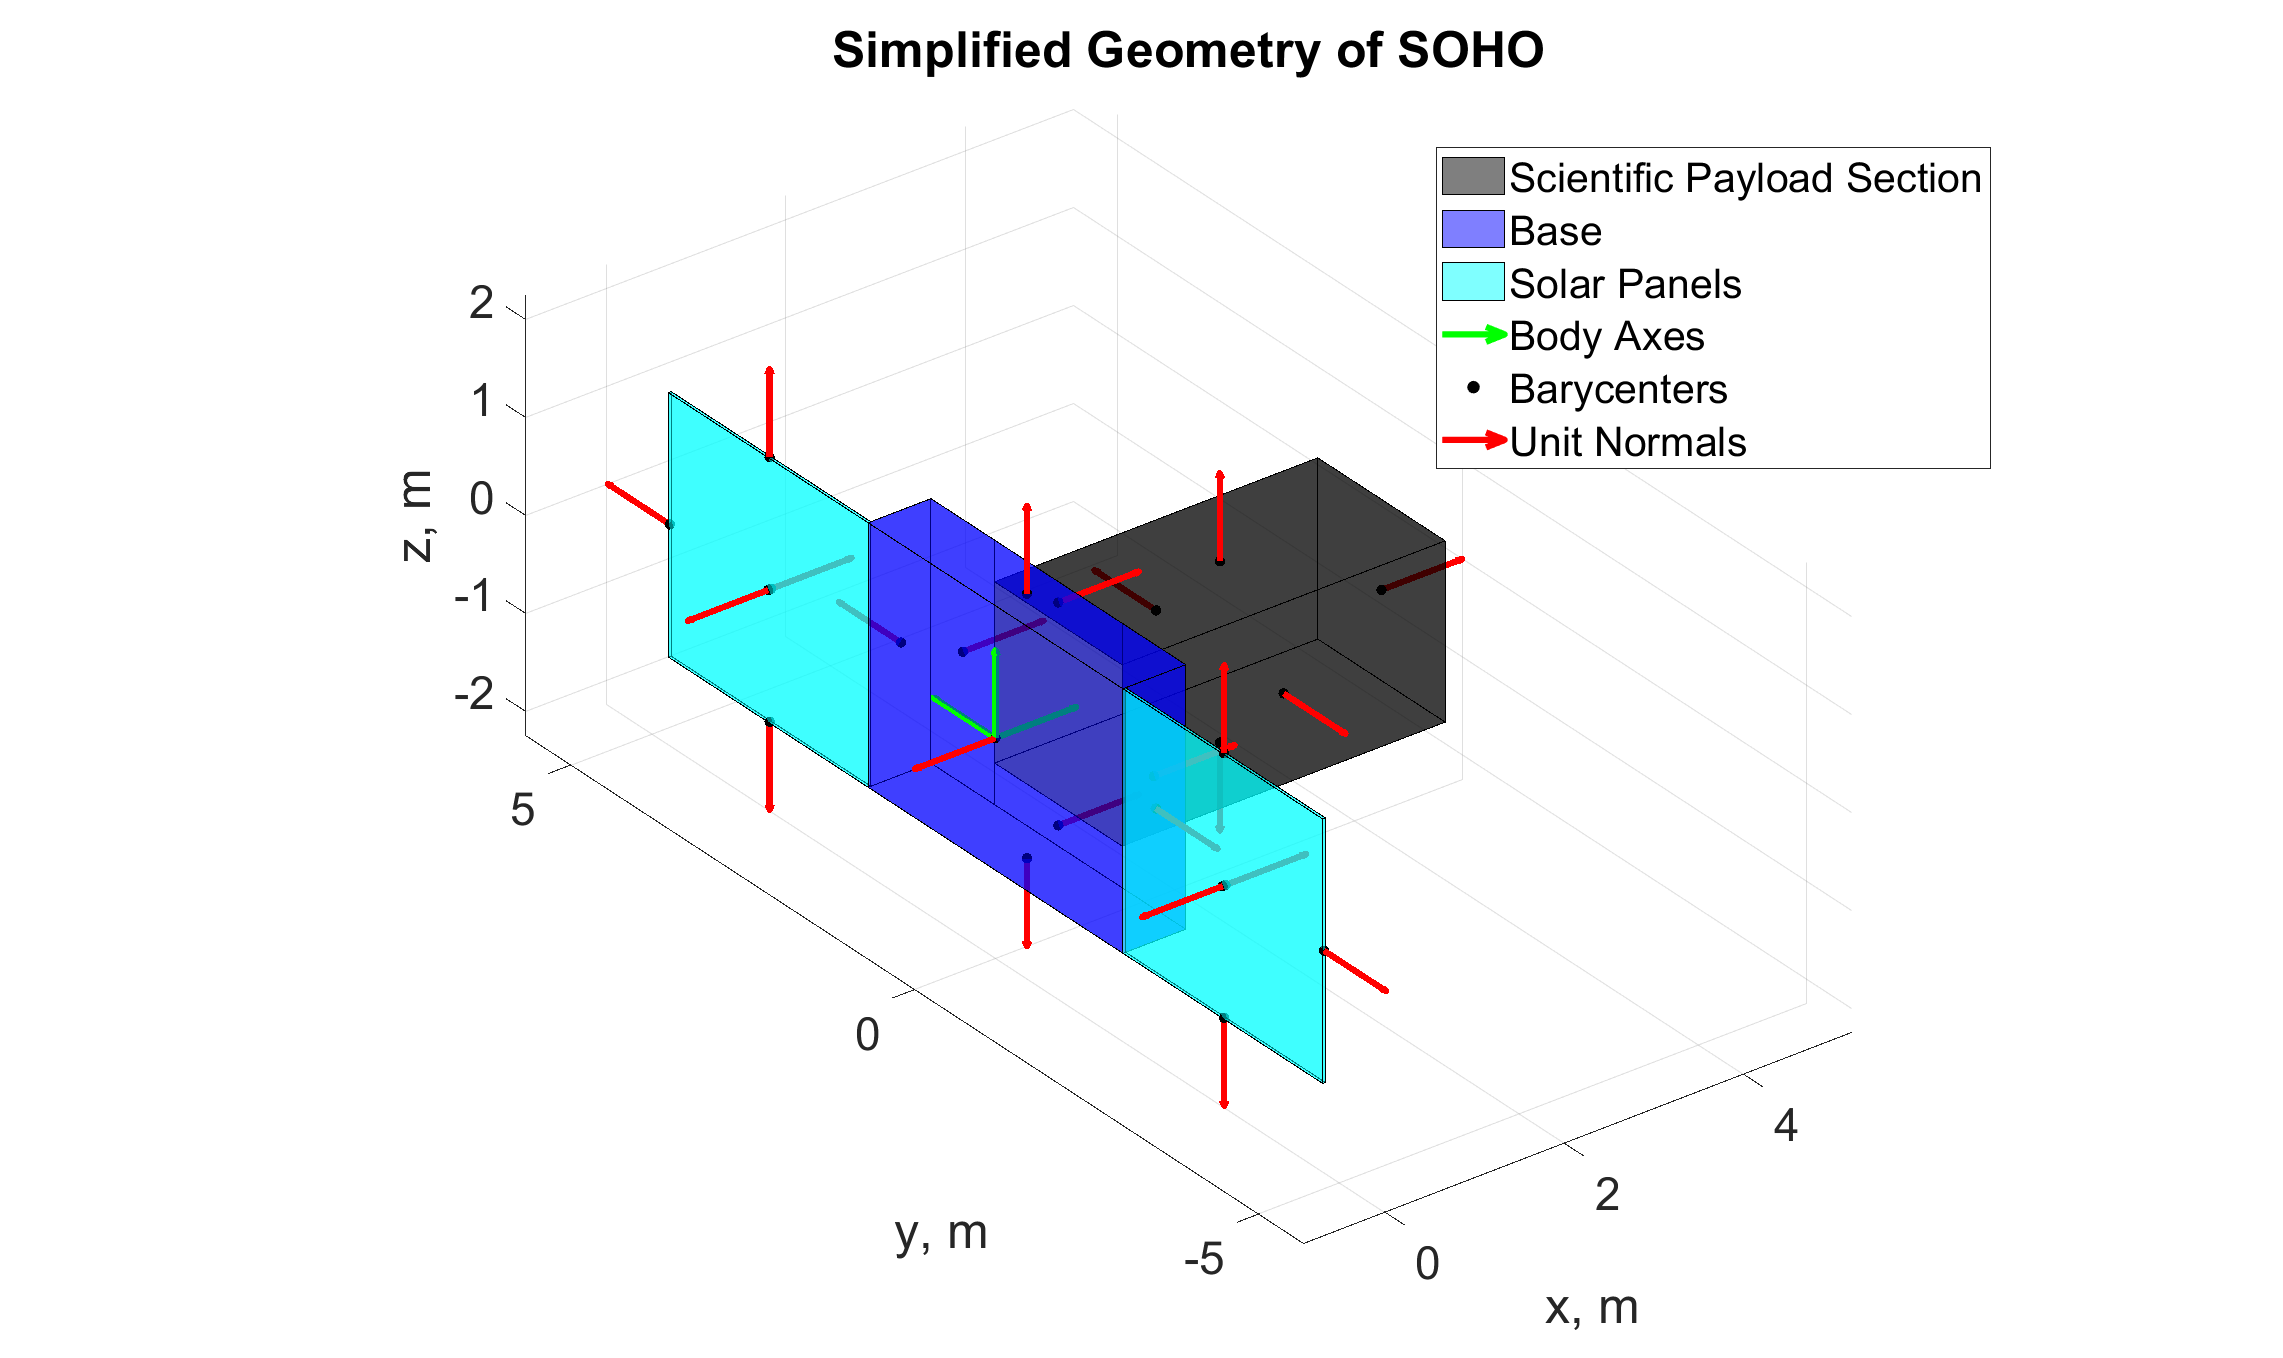
\includegraphics[width=\textwidth]{Images/SOHO_geo.eps}
  \caption{Discretized spacecraft geometry showing both the barycenters and the normal vectors of each outward face.}
  \label{fig:SOHO_disc}
\end{figure}

\subsection{PROBLEM 8}
\textit{At this stage you should have a simple 3D model of your spacecraft including geometry and mass properties of each element. This includes at least two coordinate systems, body and principal axes respectively, and the direction cosine matrix between them. Plot axes of triads in 3D superimposed to spacecraft 3D model.}

As found in Section \ref{principal_axes}, the body axes and principal axes are the same for our given spacecraft. With that in mind, in our 3D model of the spacecraft we show the body axes and principal axes as one set of axes. The direction cosine matrix would be the identity matrix as there is no transformation between the two. The 3D model of the spacecraft with dimensions included can be seen in Figure \ref{fig:SOHO_dim}. The mass allocations were discussed in Section \ref{geometry}. 

\begin{figure}[H]
  \centering
    \includegraphics[width=\textwidth]{Images/SOHO_dim.JPG}
  \caption{3D Model of SOHO with Dimensions.}
  \label{fig:SOHO_dim}
\end{figure}

\subsection{PROBLEM 9}
\textit{Define orbit initial conditions and make sure you can propagate the orbit of the satellite over multiple orbits using either a Keplerian propagator or a numerical integration scheme (see AA279A material). If you decide to use a numerical integrator, you can later try to feed the same environmental forces for orbit propagation which are applied for attitude propagation (very cool!)}

The SOHO mission, once in the science operation phase, is orbitting the L1 point of the Earth-Moon-Sun system in a halo orbit. To model this, the problem was defined as a Circular Restricted Three Body Problem (CRTBP). This allowed for simplifications to be made to the equations of motion (EOM) for the satellite. The CRTBP was then formulated to have the Sun be mass 1, and the Earth and the Moon system be mass 2. The non-dimensional EOM are then:
\begin{equation}
\begin{aligned}
    \ddot{x} &= x + 2\dot{y} - (1-\mu)\frac{x+\mu}{\rho_{1}^{3}}-\mu\frac{x-(1-\mu)}{\rho_{2}^{3}}\\
    \ddot{y} &= y - 2\dot{x} - (1-\mu)\frac{y}{\rho_{1}^{3}}-\mu\frac{y}{\rho_{2}^{3}}\\
    \ddot{z} &= -(1-\mu)\frac{z}{\rho_{1}^{3}} - \mu\frac{z}{\rho_{2}^{3}}
\end{aligned}
\end{equation}
with \(\mu\) being the mass ratio and \(\rho_{i}\) being the distance from the spacecraft to each of the large masses in the system \cite{CRTBP}. The coordinate system being used is a rotating frame located at the barycenter of the Earth-Moon-Sun system. This frame can be seen depicted in Figure \ref{fig:frame}

\begin{figure}[H]
  \centering
    \includegraphics[width=.75\textwidth]{Images/barycenterframe.JPG}
  \caption{Rotating coordinate frame located at the barycenter.}
  \label{fig:frame}
\end{figure}


The orbit was simulated using ODE 113 in Matlab. One period was propagated (~177 days) and is shown in Figures \ref{fig:halo} and \ref{fig:haloL1}. The code to generate this orbit can be found in \ref{A:P1p9}.

\begin{figure}[H]
  \centering
    \includegraphics[width=.75\textwidth]{Images/halorotating.jpg}
  \caption{Halo orbit around the L1 point in the rotating frame centered at the barycenter of the Earth-Moon-Sun system.}
  \label{fig:halo}
\end{figure}

\begin{figure}[H]
  \centering
    \includegraphics[width=.75\textwidth]{Images/haloL1.jpg}
  \caption{Different views of the Halo Orbit.}
  \label{fig:haloL1}
\end{figure}

While the orbit remains periodic for one orbit, by running for two orbit periods it can be seen that the orbit degrades in Figure \ref{fig:halo_2}. This makes sense due to the unstable nature of the L1 point so in the future we will need to apply correctional burns to stay on the nominal trajectory.

\begin{figure}[H]
  \centering
    \includegraphics[width=\textwidth]{Images/halorotating_2.jpg}
  \caption{Halo orbit degrading during the second orbit.}
  \label{fig:halo_2}
\end{figure}

\newpage
\printbibliography

\newpage
\appendix
\addappheadtotoc
\Large{\bf{\appendixname}}
\section{Matlab Code}
\subsection{PSet1 Problem 5}\label{A:P1p5}
\begin{lstlisting}
%% Inertia Tensor
close all
clear
clc
%% Constants
% Base Section
m_b = 1144.107; % mass of base
w_b = 3.7;
b_b = 2.7;
h_b = 0.7;
% Solar Panels
m_sp = 47.947; % mass of each solar panel
w_sp = 2.9;
b_sp = 2.7;
h_sp = 0.03;
% Payload Section
m_p = 610; % mass of payload section
w_p = 1.85;
b_p = 1.85;
h_p = 3.6;
%% Inertia calcs
% X-dim
I_xb = (1/12)*m_b*(w_b^2 + b_b^2);
I_xsp = (1/12)*m_sp*(w_sp^2 + b_sp^2);
d_xsp = 0.5*(w_b + w_sp);
I_xp = (1/12)*m_p*(w_p^2 + b_p^2);
% Total X-dim
I_x = I_xb + 2*(I_xsp + m_sp*(d_xsp^2)) + I_xp;
% Y-dim
I_yb = (1/12)*m_b*(b_b^2 + h_b^2);
I_ysp = (1/12)*m_sp*(b_sp^2 + h_sp^2);
I_yp = (1/12)*m_p*(b_p^2 + h_p^2);
% Total Y-dim
I_y = (I_yb + m_b * (h_b/2)^2) + 2*(I_ysp+m_sp*(h_sp/2)^2) + (I_yp+m_p*(h_p/2+h_b)^2);
% Z-dim
I_zb = (1/12)*m_b*(h_b^2 + w_b^2);
d_zb = 0.5*(h_b);
I_zsp = (1/12)*m_sp*(h_sp^2 + w_sp^2);
d_zsp = sqrt((h_sp/2)^2 + ((w_sp+w_b)/2)^2);
I_zp = (1/12)*m_p*(h_p^2 + w_p^2);
d_zp = h_b + 0.5*(h_p);
% Total Z-dim
I_z = (I_zb + m_b*(d_zb^2)) + 2*(I_zsp + m_sp*(d_zsp^2)) + (I_zp + m_p*(d_zp^2));
% Products of Inertia
I_xy = 0; % z-x plane symmetric
I_xz = 0; % x-y plane symmetric
I_zy = 0; % z-x plane symmetric
I_yx = I_xy;
I_zx = I_xz;
I_yz = I_zy;
%% Body Axes Inertia Tensor
I_b = [I_x,-I_xy,-I_xz;-I_yx,I_y,-I_yz;-I_zx,-I_zy,I_z];
%% Principal Axes Inertia Tensor
[R,I_p] = eig(I_b); % R - eigenvectors/rotation matrix, D - eigenvalues/inertia tensor principal axes
\end{lstlisting}
\subsection{PSet1 Problem 7}\label{A:P1p7}
\begin{lstlisting}
%% Satellite Generator
close all
clear all
set(0,'DefaultLineLineWidth',1.5)
set(0,'DefaultLineMarkerSize',15)
set(0,'DefaultAxesFontSize',22)
set(0,'DefaultTextFontSize',26)


%% Geometry Parameters
rect.b = 1.85;
rect.h = 3.6;
rect.w = 1.85;

base.h = 0.7;
base.w = 3.7;
base.b = 2.7;

sp.h = 0.03;
sp.w = 2.9;
sp.b = 2.7;
[sc, fig] = SOHO_gen(rect, base, sp);
[sc, fig] = barycenter_sat(sc, fig);
sc = sc_area(sc);
[sc, fig] = sc_normals(sc, fig);
\end{lstlisting}
\begin{lstlisting}
function [sc, fig] = SOHO_gen(rect,base,sp)
% Will generate structure with coordinates for the spacecraft components
%   Inputs are structs of the height, width, and breadth of the spacecraft
%   components


rectb = rect.b;
recth = rect.h;
rectw = rect.w;

baseh = base.h;
basew = base.w;
baseb = base.b;

sph = sp.h;
spw = sp.w;
spb = sp.b;

%% Rect Prism 5 faces (one attached to the hexagon)
fig = figure();
Rectf1 = vert2rect([0,0], [rectw, rectb], 1, [recth+baseh -rectw/2 -rectb/2]);
fill3(Rectf1(:,1),Rectf1(:,2),Rectf1(:,3),'k','FaceAlpha',0.5,
'HandleVisibility','off')
hold on
xlabel('x, m')
ylabel('y, m')
zlabel('z, m')
grid on
Rectf2 = vert2rect([0,0], [recth, rectb], 2, [baseh rectw/2 -rectb/2]);
fill3(Rectf2(:,1),Rectf2(:,2),Rectf2(:,3),'k','FaceAlpha',0.5,
'HandleVisibility','off')

Rectf3 = vert2rect([0,0], [recth, rectw], 3, [baseh -rectw/2 rectb/2]);
fill3(Rectf3(:,1),Rectf3(:,2),Rectf3(:,3),'k','FaceAlpha',0.5,
'HandleVisibility','off')

Rectf4 = vert2rect([0,0], [recth, rectb], 2, [baseh -rectw/2 -rectb/2]);
fill3(Rectf4(:,1),Rectf4(:,2),Rectf4(:,3),'k','FaceAlpha',0.5,
'HandleVisibility','off')

Rectf5 = vert2rect([0,0], [recth, rectw], 3, [baseh -rectw/2 -rectb/2]);
fill3(Rectf5(:,1),Rectf5(:,2),Rectf5(:,3),'k','FaceAlpha',0.5)


%% Base Rect 9 faces (square missing in middle where attaches to rect prism)
BR1 = vert2rect([0,0], [basew, baseb], 1, [0 -basew/2 -baseb/2]);
fill3(BR1(:,1),BR1(:,2),BR1(:,3),'b','FaceAlpha',0.5,
'HandleVisibility','off')

BR2 = vert2rect([0,0], [baseh-sph, baseb], 2, [sph basew/2 -baseb/2]);
fill3(BR2(:,1),BR2(:,2),BR2(:,3),'b','FaceAlpha',0.5,
'HandleVisibility','off')

BR3 = vert2rect([0,0], [baseh-sph, baseb], 2, [sph -basew/2 -baseb/2]);
fill3(BR3(:,1),BR3(:,2),BR3(:,3),'b','FaceAlpha',0.5,
'HandleVisibility','off')

BR4 = vert2rect([0,0], [baseh, basew], 3, [0 -basew/2 baseb/2]);
fill3(BR4(:,1),BR4(:,2),BR4(:,3),'b','FaceAlpha',0.5,
'HandleVisibility','off')

BR5 = vert2rect([0,0], [baseh, basew], 3, [0 -basew/2 -baseb/2]);
fill3(BR5(:,1),BR5(:,2),BR5(:,3),'b','FaceAlpha',0.5,
'HandleVisibility','off')

BR6 = vert2rect([0,0], [(basew-rectw)/2, baseb], 1, [baseh -basew/2 -baseb/2]);
fill3(BR6(:,1),BR6(:,2),BR6(:,3),'b','FaceAlpha',0.5,
'HandleVisibility','off')

BR7 = vert2rect([0,0], [(basew-rectw)/2, baseb], 1, [baseh basew/4 -baseb/2]);
fill3(BR7(:,1),BR7(:,2),BR7(:,3),'b','FaceAlpha',0.5,
'HandleVisibility','off')

BR8 = vert2rect([0,0], [rectb, (baseb-rectw)/2], 1, [baseh -basew/4 rectb/2]);
fill3(BR8(:,1),BR8(:,2),BR8(:,3),'b','FaceAlpha',0.5,
'HandleVisibility','off')

BR9 = vert2rect([0,0], [rectb, (baseb-rectw)/2], 1, [baseh -basew/4 -baseb/2]);
fill3(BR9(:,1),BR9(:,2),BR9(:,3),'b','FaceAlpha',0.5)


%% Solar Panel #1 5 faces
SP11 = vert2rect([0,0], [spw, spb], 1, [0 basew/2 -baseb/2]);
fill3(SP11(:,1),SP11(:,2),SP11(:,3),'c','FaceAlpha',0.5,
'HandleVisibility','off')

SP12 = vert2rect([0,0], [spw, spb], 1, [sph basew/2 -baseb/2]);
fill3(SP12(:,1),SP12(:,2),SP12(:,3),'c','FaceAlpha',0.5,
'HandleVisibility','off')

SP13 = vert2rect([0,0], [sph, spb], 2, [0 basew/2+spw -baseb/2]);
fill3(SP13(:,1),SP13(:,2),SP13(:,3),'c','FaceAlpha',0.5,
'HandleVisibility','off')

SP14 = vert2rect([0,0], [sph, spw], 3, [0 basew/2 baseb/2]);
fill3(SP14(:,1),SP14(:,2),SP14(:,3),'c','FaceAlpha',0.5,
'HandleVisibility','off')

SP15 = vert2rect([0,0], [sph, spw], 3, [0 basew/2 -baseb/2]);
fill3(SP15(:,1),SP15(:,2),SP15(:,3),'c','FaceAlpha',0.5)
%% Solar Panel #2 5 faces
SP21 = vert2rect([0,0], [spw, spb], 1, [0 -basew/2-spw -baseb/2]);
fill3(SP21(:,1),SP21(:,2),SP21(:,3),'c','FaceAlpha',0.5,
'HandleVisibility','off')

SP22 = vert2rect([0,0], [spw, spb], 1, [sph -basew/2-spw -baseb/2]);
fill3(SP22(:,1),SP22(:,2),SP22(:,3),'c','FaceAlpha',0.5,
'HandleVisibility','off')

SP23 = vert2rect([0,0], [sph, spb], 2, [0 -(basew/2+spw) -baseb/2]);
fill3(SP23(:,1),SP23(:,2),SP23(:,3),'c','FaceAlpha',0.5,
'HandleVisibility','off')

SP24 = vert2rect([0,0], [sph, spw], 3, [0 -basew/2-spw baseb/2]);
fill3(SP24(:,1),SP24(:,2),SP24(:,3),'c','FaceAlpha',0.5,
'HandleVisibility','off')

SP25 = vert2rect([0,0], [sph, spw], 3, [0 -basew/2-spw -baseb/2]);
fill3(SP25(:,1),SP25(:,2),SP25(:,3),'c','FaceAlpha',0.5,
'HandleVisibility','off')

axis equal
title('Simplified Geometry of SOHO')
quiver3(zeros(3,1),zeros(3,1),zeros(3,1),[1;0;0],[0;1;0],[0;0;1],
'linewidth',3,'color','r')
legend('Scientific Payload Section', 'Base', 'Solar Panels','Body Axes')

hold off

sc.rect.f1.coord = Rectf1;
sc.rect.f2.coord = Rectf2;
sc.rect.f3.coord = Rectf3;
sc.rect.f4.coord = Rectf4;
sc.rect.f5.coord = Rectf5;
sc.base.f1.coord = BR1;
sc.base.f2.coord = BR2;
sc.base.f3.coord = BR3;
sc.base.f4.coord = BR4;
sc.base.f5.coord = BR5;
sc.base.f6.coord = BR6;
sc.base.f7.coord = BR7;
sc.base.f8.coord = BR8;
sc.base.f9.coord = BR9;
sc.sp1.f1.coord = SP11;
sc.sp1.f2.coord = SP12;
sc.sp1.f3.coord = SP13;
sc.sp1.f4.coord = SP14;
sc.sp1.f5.coord = SP15;
sc.sp2.f1.coord = SP21;
sc.sp2.f2.coord = SP22;
sc.sp2.f3.coord = SP23;
sc.sp2.f4.coord = SP24;
sc.sp2.f5.coord = SP25;
end
\end{lstlisting}
\begin{lstlisting}
function [sc] = sc_area(sc)

subsections = fieldnames(sc);
poss = [1 2 3];
for subsect = subsections'
    faces = fieldnames(sc.(subsect{1}));
    for face = faces'
        coord = sc.(subsect{1}).(face{1}).coord;
        for ii = 1:size(coord,2)
            if range(coord(:,ii)) == 0
                avail = poss(poss~=ii);
                area = abs((coord(3,avail(2)) - coord(1,avail(2))) *...
                    (coord(3,avail(1)) - coord(1,avail(1))));
                sc = setfield(sc,subsect{1},face{1},'area',area);
                break
            end
        end

    end
end

end
\end{lstlisting}
\begin{lstlisting}
function [sc,fig] = barycenter_sat(sc,fig)
fig;
gcf;
hold on
subsections = fieldnames(sc);
count = 1;
for subsect = subsections'
    faces = fieldnames(sc.(subsect{1}));
    for face = faces'
        coord = sc.(subsect{1}).(face{1}).coord;
        bc = [mean(coord(:,1)),mean(coord(:,2)),mean(coord(:,3))];
        sc = setfield(sc,subsect{1},face{1},'bc',bc);
        if count == 1
            scatter3(bc(1),bc(2),bc(3),25,'y','filled','DisplayName',...
                'Barycenters')
            count = count + 1;
        else
            scatter3(bc(1),bc(2),bc(3),25,'y','filled','HandleVisibility'...
                ,'off')
        end
    end
end
end
\end{lstlisting}
\begin{lstlisting}
function [sc, fig] = sc_normals(sc, fig)
fig;
gcf;
hold on
subsections = fieldnames(sc);
count = 1;
for subsect = subsections'
    faces = fieldnames(sc.(subsect{1}));
    for face = faces'
        coord = sc.(subsect{1}).(face{1}).coord;
        for ii = 1:size(coord,2)
            if range(coord(:,ii)) == 0
                nv = zeros(3,1);
                bce = sc.(subsect{1}).(face{1}).bc;
                if sign(bce(ii) - eps) > 0
                    nv(ii) = 1;
                else
                    nv(ii) = -1;
                end
                sc = setfield(sc,subsect{1},face{1},'normal',nv);
                
                if count == 1
                    quiver3(bce(1), bce(2), bce(3),...
                        nv(1), nv(2), nv(3),'linewidth'...
                        , 3,'color','m','DisplayName','Unit Normals')
                    count = count + 1;
                else
                    quiver3(bce(1), bce(2), bce(3),...
                        nv(1), nv(2), nv(3),'linewidth'...
                        , 3,'color','m','HandleVisibility','off')
                end
                quiver3(bce(1), bce(2), bce(3),...
                    nv(1), nv(2), nv(3),'linewidth'...
                    , 3,'color','m','HandleVisibility','off')
                break
            end
        end

    end
end
end
\end{lstlisting}
\subsection{PSet1 Problem 9}\label{A:P1p9}
\begin{lstlisting}
clear all
close all
%% Problem Set 1 Problem 9
constants
%% Initial Conditions
mu1 = 328900.56^-1; % From NASA
M1 = 1 - mu1;
M2 = mu1;
omega = sqrt((mu.earth + mu.moon + mu.sun)/dis.sun^3);

%% solving L1
syms x
eqn = x - (1-mu1)/(x+mu1)^2 + mu1/(x-1+mu1)^2 == 0;
digitsOld = digits(100);
L1 = vpasolve(eqn,x,[0,1]);

highPrecisionL1 = double(L1) ;
digits(digitsOld)

%% Initial r and v
r = [.98900883730044109; 0; 0.000802140914099732];
v = [0; 0.00745547624046035; 0]; % be careful changing. Very sensitive.
state_sc_earth = [r; v; mu1];
%% solving the orbit


tstart = 0;
tint = 25*omega;
tend = 3600*24*176.9228*omega; % convert to nondimensional time

options = odeset('RelTol', 1e-3, 'AbsTol', 1e-6); 
[t_out, y_out] = ode113(@orbit_prop, [tstart:tint:tend]', state_sc_earth, options); 

%% Plotting
figure()
plot(y_out(:,1)*dis.sun, y_out(:,2)*dis.sun)
hold on
% plot(y_out(:,7), y_out(:,8))
scatter(double(L1)*dis.sun,0,25,'filled')
% scatter(mu1*dis.sun,0,25,'filled')
scatter((1-mu1)*dis.sun,0,25,'filled','b')
title('Halo Orbit around L1 in the Rotating Barycenter Frame')
xlabel('x position, km')
ylabel('y position, km')
axis equal
grid on
legend('Halo Orbit', 'L1 Point', 'Earth')
hold off
(y_out(1,1) - y_out(end,1))*dis.sun; %check on final error in the distance


figure()
plot3(y_out(:,1)*dis.sun,y_out(:,2)*dis.sun,y_out(:,3)*dis.sun)
hold on
scatter3(double(L1)*dis.sun,0,0,25,'filled')
title('Halo Orbitf')
xlabel('x position, km')
ylabel('y position, km')
zlabel('z position, km')
axis equal
grid on
hold off
\end{lstlisting}
\begin{lstlisting}
function [statedot] = orbit_prop(t, state)
% state is [r_3 v_3 mu]
%   although required by form, t will be unused


statedot = zeros(7,1);
x = state(1);
y = state(2);
z = state(3);
xdot = state(4);
ydot = state(5);
zdot = state(6);

mu = state(7);

rho1 = sqrt((x + mu)^2 + y^2 + z^2);
rho2 = sqrt((x - (1-mu))^2 + y^2 + z^2);

statedot(1) = xdot;
statedot(2) = ydot;
statedot(3) = zdot;

statedot(4) = x + 2*ydot - (1 - mu)*(x + mu)/rho1^3 - ...
    mu*(x - (1 - mu))/rho2^3;
statedot(5) = y - 2*xdot - (1 - mu)*(y)/rho1^3 - ...
    mu*(y)/rho2^3;
statedot(6) = -(1 - mu)*z/rho1^3 - mu*z/rho2^3;
for ii = 4:6
    if abs(statedot(ii)) < 1e-15
        statedot(ii) = 0;
    end
end
end
\end{lstlisting}



\end{document}